\documentclass[12pt]{article}
\usepackage[letterpaper,margin=.65in,headheight=18pt,headsep=18pt,footskip=25pt]{geometry}
\usepackage[T1]{fontenc}\usepackage{helvet}\renewcommand{\familydefault}{\sfdefault}
\usepackage{tikz,array,fancyhdr}\usetikzlibrary{arrows.meta}
\pagestyle{fancy}\fancyhf{}\renewcommand{\headrulewidth}{0pt}
\fancyhead[L]{\small Week 30 / Weight kits encore / Grades 2--5}
\fancyfoot[L]{\scriptsize Bellingham Math Circle / Week 30 / W30-BON-v1}\fancyfoot[R]{\scriptsize\thepage}
\setlength{\parindent}{0pt}\setlength{\parskip}{9pt}
\newcommand{\problem}[2]{\par\textbf{Problem #1:} #2\par}
\newcommand{\blank}[1]{\vspace{#1}}
\newcommand{\cards}[1]{\begin{tikzpicture}[x=1.4cm,y=1cm]\foreach \n [count=\i from 0] in {#1}{\draw (\i,0) rectangle +(1.05,.85);\node at (\i+.525,.425){\Large\n};}\end{tikzpicture}}
\begin{document}
Weights are positive whole amounts. A card cannot be split or used twice. The target stays on the left pan. Put a weight on either pan or leave it off.

\problem{1}{Use the kit $1,2,3$. Your partner removes one weight. Balance each target $1,2,3$ with the weights that remain. Find balances for every possible removal.}
\begin{center}\cards{1,2,3}\end{center}
\begin{center}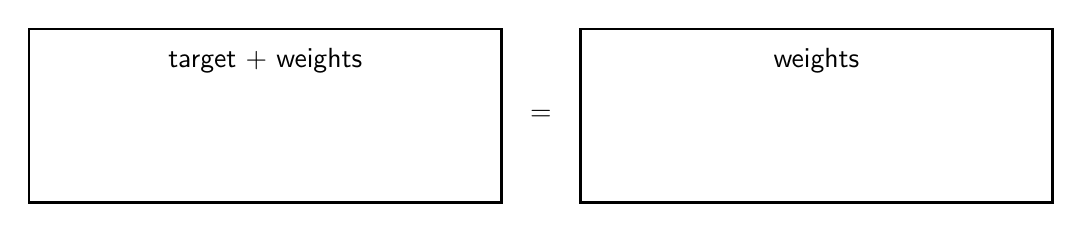
\begin{tikzpicture}[x=1cm,y=1cm]
\draw[line width=1pt] (0,0) rectangle (6,2.2);\draw[line width=1pt] (7,0) rectangle (13,2.2);
\node at (3,1.8){target + weights};\node at (10,1.8){weights};
\node at (6.5,1.1){$=$};
\end{tikzpicture}\end{center}
\renewcommand{\arraystretch}{1.75}
\begin{center}\begin{tabular}{|c|c|p{3.9cm}|p{3.9cm}|}\hline
Removed & Target & Left-pan weights & Right-pan weights\\\hline
1&1&&\\\hline 1&2&&\\\hline 1&3&&\\\hline
2&1&&\\\hline 2&2&&\\\hline 2&3&&\\\hline
3&1&&\\\hline 3&2&&\\\hline 3&3&&\\\hline
\end{tabular}\end{center}
\newpage
\problem{2}{Choose three different weights from $1$ to $8$. Your partner may remove any one of them before choosing a target. Make a kit that can still balance every target from $1$ to $3$. Can a different kit do this?}
\begin{center}\cards{1,2,3,4,5,6,7,8}\end{center}
\begin{center}\begin{tikzpicture}\foreach \x in {0,2.5,5}{\draw (\x,0) rectangle +(1.6,1.4);}\end{tikzpicture}\end{center}
\blank{1.0cm}
\problem{3}{Can three different whole-number weights still balance every target from $1$ to $4$ after any one weight is removed? Choose weights of any size. Find a kit or explain why no kit can work.}
\blank{8cm}
\newpage
Compare a hidden mass with any known whole-number mass. Your partner answers \emph{lighter}, \emph{equal}, or \emph{heavier}. Guessing the only remaining candidate uses no comparison.

\begin{center}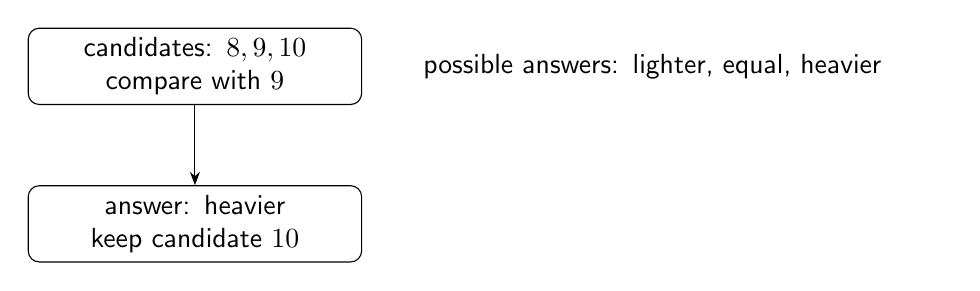
\begin{tikzpicture}[x=1cm,y=1cm,>=Stealth]
\node[draw,rounded corners,text width=4.0cm,align=center] (a) at (0,0){candidates: $8,9,10$\\compare with $9$};
\node[text width=6.6cm,align=left] (b) at (6.2,0){possible answers: lighter, equal, heavier};
\node[draw,rounded corners,text width=4.0cm,align=center] (c) at (0,-2.0){answer: heavier\\keep candidate $10$};
\draw[->] (a)--(c);
\end{tikzpicture}\end{center}
\problem{4}{Your partner hides one card from $1$ to $7$. Make a plan that always finds it in at most two comparisons. Test your plan with your partner using each possible hidden card.}
\blank{4.6cm}
\begin{center}\cards{1,2,3,4,5,6,7}\end{center}
\problem{5}{Could a plan always find a hidden card from $1$ to $8$ in at most two comparisons? Explain your answer.}
\blank{2.5cm}
\newpage
For teams, use every listed weight once. Each team needs at least one weight. All team totals must match.
\problem{6}{Put each kit into the requested number of equal-weight teams. If a kit cannot be divided that way, explain why.}
\renewcommand{\arraystretch}{2}
\begin{center}\begin{tabular}{p{4cm}p{10cm}}
Kit $1,2,3,4$\newline 2 teams & \begin{tikzpicture}\foreach \x in {0,4.1}{\draw (\x,0) rectangle +(3.6,1.5);}\end{tikzpicture}\\[9mm]
Kit $1,2,3,4,5,6$\newline 3 teams & \begin{tikzpicture}\foreach \x in {0,2.7,5.4}{\draw (\x,0) rectangle +(2.3,1.5);}\end{tikzpicture}\\[9mm]
Kit $1,2,5$\newline 2 teams & \begin{tikzpicture}\foreach \x in {0,4.1}{\draw (\x,0) rectangle +(3.6,1.5);}\end{tikzpicture}\\[9mm]
Kit $1,2,3,4,5,6,7,8$\newline 4 teams & \begin{tikzpicture}\foreach \x in {0,2,4,6}{\draw (\x,0) rectangle +(1.7,1.5);}\end{tikzpicture}\\
\end{tabular}\end{center}
\blank{1cm}
\problem{7}{Find every way to split $1,2,3,4,5,6$ into three equal-weight teams. Moving a whole team to another tray does not make a new way.}
\blank{3cm}
\end{document}
